% This is "sig-alternate.tex" V2.0 May 2012
% This file should be compiled with V2.5 of "sig-alternate.cls" May 2012
%
% This example file demonstrates the use of the 'sig-alternate.cls'
% V2.5 LaTeX2e document class file. It is for those submitting
% articles to ACM Conference Proceedings WHO DO NOT WISH TO
% STRICTLY ADHERE TO THE SIGS (PUBS-BOARD-ENDORSED) STYLE.
% The 'sig-alternate.cls' file will produce a similar-looking,
% albeit, 'tighter' paper resulting in, invariably, fewer pages.
%
% ----------------------------------------------------------------------------------------------------------------
% This .tex file (and associated .cls V2.5) produces:
%       1) The Permission Statement
%       2) The Conference (location) Info information
%       3) The Copyright Line with ACM data
%       4) NO page numbers
%
% as against the acm_proc_article-sp.cls file which
% DOES NOT produce 1) thru' 3) above.
%
% Using 'sig-alternate.cls' you have control, however, from within
% the source .tex file, over both the CopyrightYear
% (defaulted to 200X) and the ACM Copyright Data
% (defaulted to X-XXXXX-XX-X/XX/XX).
% e.g.
% \CopyrightYear{2007} will cause 2007 to appear in the copyright line.
% \crdata{0-12345-67-8/90/12} will cause 0-12345-67-8/90/12 to appear in the copyright line.
%
% ---------------------------------------------------------------------------------------------------------------
% This .tex source is an example which *does* use
% the .bib file (from which the .bbl file % is produced).
% REMEMBER HOWEVER: After having produced the .bbl file,
% and prior to final submission, you *NEED* to 'insert'
% your .bbl file into your source .tex file so as to provide
% ONE 'self-contained' source file.
%
% ================= IF YOU HAVE QUESTIONS =======================
% Questions regarding the SIGS styles, SIGS policies and
% procedures, Conferences etc. should be sent to
% Adrienne Griscti (griscti@acm.org)
%
% Technical questions _only_ to
% Gerald Murray (murray@hq.acm.org)
% ===============================================================
%
% For tracking purposes - this is V2.0 - May 2012

\documentclass{acm_proc_article-me}
\graphicspath{{IMAGES/}}



\usepackage{xspace}
\usepackage{color}

\newcommand{\mypartitle}[2][2.5]{\vspace*{-#1 ex}~\\{\noindent {\bf #2}}}
\newcommand{\mypartitleit}[2][2]{\vspace*{-#1 ex}~\\{\noindent {\it #2}}}
\newcommand{\mypartitletwo}[1]{\vspace*{-3ex}~\\{\noindent \underline{#1}}}

\newcommand{\mycite}[1]{{\cite{#1}}}
\newcommand{\degree}{\ensuremath{^\circ}\xspace}

\newcommand{\mycomment}[1]{{{ \color{red} #1 }}}
%\newcommand{\mycomment}[1]{{{ \uppercase{#1} }}}
%\newcommand{\mycomment}[1]{}

%%%%%%%%%%%%%%%%%%%%%%%%%%%%%%%%%%%%%%%%%%%%%%%
%%% CLUSTERING VARIABLES
%%%%%%%%%%%%%%%%%%%%%%%%%%%%%%%%%%%%%%%%%%%%%%%

\newcommand{\SurfClusterDistance}{\ensuremath{D_{S}}\xspace}
\newcommand{\DCTset}{\ensuremath{\mathbf{O}}\xspace}
\newcommand{\DCTvec}{\ensuremath{\mathbf{o}}\xspace}
\newcommand{\UBMmean}{\ensuremath{\mathbf{m}}\xspace}
\newcommand{\IDmean}{\ensuremath{\mathbf{s}}\xspace}
\newcommand{\IDUBMoffset}{\ensuremath{\mathbf{d}}\xspace}
\newcommand{\Ivector}{\ensuremath{\mathbf{u}}\xspace}
\newcommand{\TVsubspace}{\ensuremath{T}\xspace}
\newcommand{\TVnoise}{\ensuremath{\xi}\xspace}
\newcommand{\TVcova}{\ensuremath{\Sigma_{T\!v}}\xspace}
\newcommand{\TVfirstorder}{\ensuremath{F}\xspace}
\newcommand{\TVzeroorder}{\ensuremath{N}\xspace}
\newcommand{\IvectorDistance}{\ensuremath{D_{T}}\xspace}

\newcommand{\ThreshLocal}{\ensuremath{Th_{1}}\xspace}
\newcommand{\ThreshSurf}{\ensuremath{Th_{2}}\xspace}
\newcommand{\ThreshFinal}{\ensuremath{Th_{3}}\xspace}


%%%%%%%%%%%%%%%%%%%%%%%%%%%%%%%%%%%%%%%%%%%%%%%
%%% TRACKING VARIABLES
%%%%%%%%%%%%%%%%%%%%%%%%%%%%%%%%%%%%%%%%%%%%%%%

%\newcommand{\position}{\ensuremath{\bf{x}}\xspace}
%\newcommand{\position}{\ensuremath{X}\xspace}
\newcommand{\position}{\ensuremath{\mathbf{x}}\xspace}
\newcommand{\displacement}{\ensuremath{\mathbf{d}}\xspace}
\newcommand{\imageposition}{\ensuremath{\mathbf{x}^{im}}\xspace}
\newcommand{\colorhist}{\ensuremath{\mathbf{h}}\xspace}
\newcommand{\partset}{\ensuremath{{\cal P}}\xspace}
%\newcommand{\partset}{\ensuremath{P}\xspace}
\newcommand{\motion}{\ensuremath{\mathbf{v}}\xspace}

\newcommand{\pairset}{\ensuremath{\mathbf{{\cal V}}}\xspace}
\newcommand{\timediff}{\ensuremath{\mathbf{{\Delta}}}\xspace}

\newcommand{\bydef}{\ensuremath{\stackrel{\Delta}{=}}\xspace}


\newcommand{\detlabel}{\ensuremath{l}\xspace}
\newcommand{\labelfield}{\ensuremath{L}\xspace}
\newcommand{\detectionset}{\ensuremath{Y}\xspace}
\newcommand{\detection}{\ensuremath{y}\xspace}
\newcommand{\dettime}{\ensuremath{t}\xspace}
\newcommand{\featurefct}{\ensuremath{S}\xspace}
\newcommand{\confidencescore}{\ensuremath{w}\xspace}
%\newcommand{\confidenceset}{\ensuremath{\mathbf{W}}\xspace}
\newcommand{\confidenceset}{\ensuremath{{\cal W}}\xspace}


\newcommand{\param}{\ensuremath{\lambda}\xspace}
\newcommand{\paramk}{\ensuremath{\param^{r}}\xspace}
\newcommand{\parampos}{\ensuremath{\param^{1}}\xspace}
\newcommand{\paramcol}{\ensuremath{\param^{2}}\xspace}
\newcommand{\npcol}{\ensuremath{\alpha}\xspace}
\newcommand{\npmotion}{\ensuremath{\alpha}\xspace}
\newcommand{\paramkdel}[1]{\ensuremath{\param^{k}_{#1}}\xspace}
\newcommand{\paramposdel}[1]{\ensuremath{\param^{1}_{#1}}\xspace}
\newcommand{\paramcoldel}[1]{\ensuremath{\param^{2}_{#1}}\xspace}

\newcommand{\posset}{\ensuremath{{\mathcal{P}}}\xspace}
\newcommand{\closestset}{\ensuremath{{\mathcal{C}^{\star}}}\xspace}
%\newcommand{\secondset}{\ensuremath{{\mathcal{S}_{\Delta}}}\xspace}
\newcommand{\secondset}{\ensuremath{{\mathcal{S}^{\star}}}\xspace}
\newcommand{\closestsettracklets}{\ensuremath{{\mathcal{C}}}\xspace}
\newcommand{\secondsettracklets}{\ensuremath{{\mathcal{S}}}\xspace}
\newcommand{\colsetzero}{\ensuremath{{\mathcal{C}_{\Delta,H_0}}}\xspace}
\newcommand{\colsetone}{\ensuremath{{\mathcal{C}_{\Delta,H_1}}}\xspace}

\newcommand{\closestsetdeltastar}{\ensuremath{{\mathcal{C}_{\timediff}^{\star}}}\xspace}
\newcommand{\secondsetdeltastar}{\ensuremath{{\mathcal{S}_{\timediff}^{\star}}}\xspace}

\newcommand{\Ngauss}{\ensuremath{N_{mix}}\xspace}


\newcommand{\Ndetections}{\ensuremath{N_{y}}\xspace}
%\newcommand{\Npairwisefct}{\ensuremath{N_2}\xspace}
\newcommand{\Npairwisefct}{\ensuremath{N_{s}}\xspace}
\newcommand{\Nunitaryfct}{\ensuremath{N_1}\xspace}
\newcommand{\Nfeature}{\ensuremath{N_{f}}\xspace}
%\newcommand{\Tshort}{\ensuremath{T_{short}}\xspace}
\newcommand{\Tshort}{\ensuremath{T_{w}}\xspace}

\newcommand{\meanmult}{\ensuremath{{\bf{m}}}\xspace}




\newcommand{\sigmoid}{\ensuremath{{S}}\xspace}

\newcommand{\uniquelabel}{\ensuremath{{\cal U}}\xspace}
\newcommand{\coeflabelfield}{\ensuremath{\rho}\xspace}
\newcommand{\trackcost}{\ensuremath{{C}}\xspace}
\newcommand{\trackcoststart}{\ensuremath{{C}^s}\xspace}
\newcommand{\trackcostend}{\ensuremath{{C}^e}\xspace}
\newcommand{\trackset}{\ensuremath{{\cal \tau}}\xspace}
\newcommand{\tracklet}{\ensuremath{{\tau}}\xspace}
\newcommand{\tstart}{\ensuremath{{t}^s}\xspace}
\newcommand{\tend}{\ensuremath{{t}^e}\xspace}
\newcommand{\timemargin}{\ensuremath{\theta_{tm}}\xspace}
\newcommand{\trackduration}{\ensuremath{{d}}\xspace}
\newcommand{\trackdurationmax}{\ensuremath{{d_{\max}}}\xspace}


\newcommand{\cueconfidence}{\ensuremath{{c}}\xspace}


\newcommand{\parapositionconf}{\ensuremath{{\theta_f}}\xspace}


\newcommand{\assomatrixsl}{\ensuremath{\mathbf{A}^{SW}}\xspace}
\newcommand{\assomatrixbicm}{\ensuremath{\mathbf{A}^{BI}}\xspace}
\newcommand{\Nblockb}{\ensuremath{N^{B}_{\tau}}\xspace}
\newcommand{\Nblocka}{\ensuremath{N^{A}_{\tau}}\xspace}

\newcommand{\labelfieldactive}{\ensuremath{L_a}\xspace}


\endinput

%\newcommand{\mypartitle}[2][2]{\vspace*{-#1 ex}~\\{\noindent {\bf #2}}}

\usepackage{amssymb}
\usepackage{amsfonts}
\usepackage{url}
\usepackage{paralist}

\begin{document}
%
% --- Author Metadata here ---
%\conferenceinfo{\textit{MediaEval 2015 Workshop,}}{Sept. 14-15, 2015, Wurzen, Germany}
%\CopyrightYear{2007} % Allows default copyright year (20XX) to be over-ridden - IF NEED BE.
%\crdata{0-12345-67-8/90/01}  % Allows default copyright data (0-89791-88-6/97/05) to be over-ridden - IF NEED BE.
% --- End of Author Metadata ---

\title{(Provisional) Towards large scale multimedia indexing: A case study in person discovery in broadcast news\\[-100mm]}
%
% We need to keep anonymity for the reviewers
%\author{Nam Le$^{1, 2}$, Alexander Heili$^{1}$, Di Wu$^{1}$, Jean-Marc Odobez$^{1, 2}$\\

\author{}
%% \author{Author 1$^{1, 2}$, Author 2$^{1}$, Author 3$^{1, 2}$\\
%% {\footnotesize %$^1$ \affaddr{Idiap Research Institute, Martigny, Switzerland}}\\
%% $^1$ \affaddr{Affiliation address 1}}\\
%% {\footnotesize %$^2$ \affaddr{\'{E}cole Polytechnique F\'{e}d\'{e}ral de Lausanne, Switzerland}}\\
%% $^2$ \affaddr{Affiliation address 2}}\\
%% %{\footnotesize \email{\{nle, aheili, dwu, odobez\}@idiap.ch}}
%% {\footnotesize \email{\{author1, author2, author3\}@mail.com}}
%% }

\maketitle


\begin{abstract}
\vspace*{-1mm}
TBA - Joint paper of Person Discovery consortiumm.
\end{abstract}

\endinput


\section{Introduction}

TV archives maintained by national institutions such as the French INA, the Netherlands Institute for Sound \& Vision, or the British Broadcasting Corporation are rapidly growing in size. The need for applications that make these archives searchable has led researchers to devote concerted effort to developing technologies that create indexes.

Because human nature leads people to be very interested in other people.
Indexes that represent the location and identity of people in the archive are indispensable for searching archives.
%
To this end, started in 2011, the REPERE challenge aimed at supporting research on multimodal person recognition~\cite{BERNARD--SLAM--2013, KAHN--CBMI--2012}. Its main goal was to answer the two questions \emph{``who speaks when?''} and \emph{``who appears when?''} using any available source of information (including pre-existing biometric models and person names extracted from text overlay and speech transcripts). 
%
Thanks to this challenge and the associated multimodal corpus~\cite{GIRAUDEL--LREC--2012}, significant progress was achieved in either supervised or unsupervised multimodal person recognition~\cite{BECHET--INTERSPEECH--2014, BENDRIS--CBMI--2013, BREDIN--ODYSSEY--2014, BREDIN--INTERSPEECH--2013, BREDIN--SLAM--2013, BREDIN--IJMIR--2014, FAVRE--SLAM--2013, GAY--CBMI--2014, POIGNANT--ASLP--2015, POIGNANT--SLAM--2013, POIGNANT--INTERSPEECH--2012, POIGNANT--MTAP--2015, ROUVIER--CBMI--2014}.

However, when the content is created or broadcast, it is not always possible to predict which people will be the most important to find in the future and biometric models may not yet be available at indexing time The goal of this task is thus to address the challenge of indexing people in the archive under real-world conditions, \emph{i.e.} when there is no pre-set list of people to index.
%
To emphasize on the importance of unsupervised person discovery, a ``Multimodal Person Discovery in Broadcast TV'' task was proposed \cite{POIGNANT--MEDIAEVAL--2015,tocite}. In this task, participants are provided with a collection of TV broadcast recordings pre-segmented into shots. Each shot $s \in \shots$ has to be automatically tagged with the names of people both speaking and appearing at the same time during the shot.
%
Because the list of people is not provided in advance, their names have to be found in the audio (\emph{e.g.}, using speech transcription -- ASR) or visual (\emph{e.g.}, using optical character recognition -- OCR) streams.
%
This makes the task completely unsupervised (\emph{i.e.} using algorithms not relying on pre-existing labels or biometric models).

In order to successfully tag the shots with the correct identities, one must find a way to assign a name correctly to a presence of the corresponding person, then that name must also be propagated to all the shots during which that person appears and speaks. For this purpose, there are 3 possible approaches:
\begin{compactitem}
\item{Clustering-based name assignment: Face/speech tracks are first aggregated into homogeneous clusters according to person identities. Then each clusters is tagged with the most probable person name.}
\item{Verification-based name propagation: A person name is first assigned to the most probable face/speech track. The name is then propagated to all face/speech tracks which are verified to have the same identity.}
\item{Graph-based name propagation: A graph is built with a face/speech track as a node and weight of edges is the similarity. Some nodes are initially tagged with the names. Names are then propagated along the edges within the graph.}
\end{compactitem}

Although these approaches share some common components in face / speech representation, each has charateristic ...

In this paper, the authors investigate all 3 approaches with their variations.
\endinput


%\section{Related Work}
\label{sec:related_work}

TBA

\endinput



%\section{Overview}

Given the raw TV broadcasts, each shot must be automatically tagged with the name(s) of people who can be both seen as well as heard in the shot along with the confident score. The list of people is not known apriori and their names must be discovered from video text overlay or speech transcripts~\cite{bredin2016mediaeval}. 
%
To this end, a video must be segmented in an unsupervised way into homogeneous segments according to person identity, like  speaker diarization and face diarization, to be combined with the extracted names.
% . Combined with the extracted names,  audio-visual person diarization makes it possible to identify people in videos. % \cite{Gay:Frontiers:2016}.
%

%\begin{figure}[tb]
%\centering
%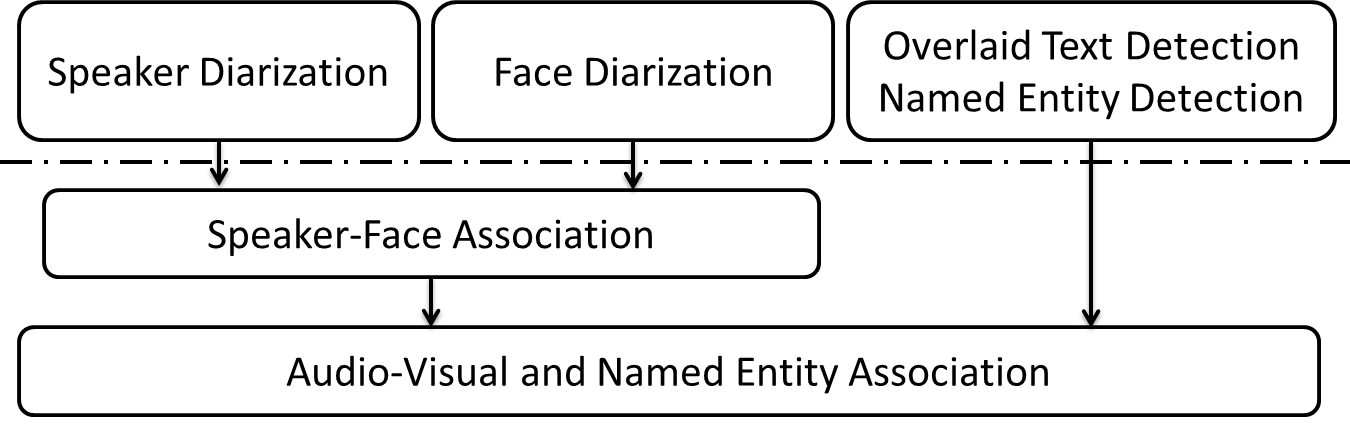
\epsfig{file=diagram.png,width=70mm}
%\vspace*{-3mm}
%\caption{Architecture of our system}
%\vspace*{-3mm}
%\label{fig:pipeline}
%\end{figure}

The overall system is illustrated in Fig.~\ref{fig:pipeline}. It consists of  4 main parts: video optical character recognition (OCR) and named entity recognition (NER), face diariation, speaker diarization, and fusion naming. Each of these parts will be described in the following sections.

\endinput


\section{Video OCR and NER}
\label{sec:ocr_ner}

Person identities can be retrieved either from speech transcripts or from overlaid person names commonly used to introduce the current speaker. Person identities from transcripts deteriorates when transcripts come from automatic speech recognition. Meanwhile, text can be reliably extracted using OCR techniques, and their association with people in the videos is easier than analysing whether or not pronounced names in ASR transcripts actually refer to people appearing in the video. Thus, in this work we use only names coming from OCR segments in videos.

To detect OCR segments in videos and exploit them for retrieval, we first relied on the approaches described in \cite{chen-pr04,odobez-prl05} for text recognition in videos, and on \cite{daddaoua:ICDAR:05,vincia:tmm:05} for text recognition and indexing.
%
In brief, given an input video, two main steps are applied: first the video is preprocessed with a motion filtering to reduce noise, and individual frames are processed to localize and binarize the text regions for text recognition.
%
As compared to printed documents, OCR in TV news videos encounters several challenges: low resolution of text regions, sequence of different texts continuously displayed, or small amount of text to be recognized etc.
%
To tackle these, multiple image segmentations of the same text region are decoded, and then all results are compared and aggregated over time to produce several hypotheses. 
%Due to the long running time, only the lower half of the videos are processed.
%
The best hypothesis is used to extract people names for identification. To recognize names from texts, we use the MITIE open library~\footnote{https://github.com/mit-nlp/MITIE}, which provides state-of-the-art NER tool. 
%
%However, detecting names for identification can be more challenging due to several factors: (a) OCR text are often not sentences but short phrases, (b) names come from various languages, and (c) there are names of editorial staff who do not appear within the video, thus are not useful for identification such as cameramen or editors.
%
To improve the raw MITIE results, a heuristics preprocessing step identifies names of editorial staff based on their roles (cameraman, editor, or writer) because they do not appear within the video, thus are not useful for identification.

\endinput


\section{Face clustering}
\label{sec:face_clustering}

\subsection{First system}

Face tracking-by-detection is applied within each shot using a detector based on histogram of oriented gradients~\cite{Dalal2005} and the correlation tracker proposed by \emph{Danelljan et al.}~\cite{Danelljan2014}. Each face track is then described by its average \emph{FaceNet} embedding and compared with all the others using Euclidean distance~\cite{Schroff2015}. Finally, average-link hierarchical agglomerative clustering is applied. Source code for this module is available in \emph{pyannote-video}\footnote{\url{http://pyannote.github.io}}.

\subsection{Second system}

A fast version of deformable part-based model (DPM)~\cite{felzenszwalb2010dpm,mathias2014face,dubout2013deformable} is first applied. Then tracking is performed using the CRF-based multi-target tracking framework~\cite{heili2014tracking}, which relies on the unsupervised learning of time sensitive association costs for different features.
%
The detector is only applied 4 times per second and an explicit false alarm classifier at the track level is learned\cite{Le_ICPR_2016}.
%
Each face track is then described using a combination of keypoint matching distances and total variability modeling (TVM)~\cite{wallace2011inter,wallace2012total,Khoury:ICMR:2013}.

\endinput


\section{Speaker Diarization}
\label{sec:speaker_diarization}

TBA

\endinput


\section{Naming}
\label{sec:naming}

TBA

\subsection{Single modal name propagation}

TBA

\subsection{Multi-modal name propagation}

TBA

\endinput


\section{Experiments}
\label{sec:experiment}
%
\subsection{Datasets and Metric}

The 2015 test corpus serves as development set for this year's task. It contains 106 hours of video, corresponding to 172 editions of evening broadcast news \emph{``Le 20 heures''} of the French public channel \emph{``France 2''}, from January 1st 2007 to June 30st 2007. This development set is associated with \emph{a posteriori} annotations based on last year participants' submissions.

The test set is divided into three datasets: INA, DW and 3-24. The INA dataset contains a full week of broadcast for 3 TV channels and 3 radio channels in French. Only a subset (made of 2 TV video channels for a total duration of 90 hours) needs to be processed. However, participants can process the rest of it if they think it might lead to improved results. Moreover, this dataset is associated with manual metadata provided by INA in the shape of CSV files. The DW dataset~\cite{EUMSSI} is composed of video downloaded from Deutsche Welle website, in English and German for a total duration of 50 hours. This dataset is also associated with metadata that can be used in contrastive runs. The last dataset contains 13 hours of broadcast from 3/24 Catalan TV news channel.

As the test set comes completely free of any annotation, it will be annotated \emph{a posteriori} based on participants' submissions.
In order to ease this annotation process, participants are asked to justify their assertion. To this end, each hypothesized name $n \in \hypNames$ has to be backed up by a carefully selected and unique shot prooving that the person actually holds this name $n$: we call this an evidence. In real-world conditions, this evidence would help a human annotator double-check the automatically-generated index, even for people they did not know beforehand.

Two types of evidence are allowed: an \emph{image} evidence is a time in a video when a person is visible, while his/her name is written on screen; an \emph{audio} evidence is the time when the name of a person is pronounced, provided that this person is visible in a $[\text{time} - 5s, \text{time} + 5s ]$ neighborhood.
For instance, in Figure~\ref{fig:evidence}, shot \#1 contains an \emph{image} evidence for Mr A (because his name and his face are visible simultaneously on screen) while shot \#3 contains an \emph{audio} evidence for Mrs B (because her name is pronounced less than 5 seconds before or after her face is visible on screen).

Because of limited resources dedicated to collaborative annotation, the test set cannot be fully annotated. Therefore, the task is evaluated indirectly as an information retrieval task, using the folllowing principle.

For each query $q \in \queries \subset \refNames$ (\texttt{first\-name\_lastname}), returned shots are first sorted by the edit distance between the hypothesized person name and the query $q$ and then by confidence scores.
Average precision $\text{AP}(q)$ is then computed classically based on the list of relevant shots (according to the groundtruth) and the sorted list of shots. Finally, Mean Average Precision is computed as follows:
\begin{align}
            \text{MAP} & = \frac{1}{|\queries|} \sum_{q \in \queries} \text{AP}(q) \nonumber
\end{align}

\subsection{Evaluation}

\begin{compactitem}
	\item Sub. (2) used our face naming without talking score with our OCR-NER.
	\item Sub. (3) used our face naming with talking score. 
	\item Sub. (4) used the combination of talking face naming in sub. (3) with speaker naming.
\end{compactitem}

\begin{table}[tb]
\centering
\begin{tabular}{c|c|c|c|}
\cline{2-4}
                                & MAP@1  & MAP@10 & MAP@100  \\ \hline

 \multicolumn{1}{|c|}{Sub. (2)} & 62.3   & 50.3   & 49.2 \\ \hline
 \multicolumn{1}{|c|}{Sub. (3)} & 69.3   & 57.0   & 55.8 \\ \hline
 \multicolumn{1}{|c|}{Sub. (4)} & 73.6   & 59.8   & 57.9 \\ \hline

\end{tabular}
\vspace*{-2mm}
\caption{Benchmarking results of our submissions. Details of each submission in the text.}
\vspace*{-2mm}
\label{tab:mediaeval}
\end{table}


%BEGINNING results IRISA/PUCMINAS---------------------------------------------------
\begin{table}[!t]
\caption{Mean average precisions @K obtained on the development and test sets using approaches by IRISA - PUC Minas. {\it no prop.}: no tag propagation. MST: tag propagation using the Minimum-Spanning Tree approach. RW: tag propagation using the Random Walk approach.}
\label{table_example}
\centering
\begin{tabular}{|c||c|c|c|c|}
% results on the development set
\multicolumn{5}{ c }{Dev16}\\
\hline
 & \multicolumn{4}{| c |}{MAP@K (\%)}\\
\hline
K  & 1 & 5 & 10 & 100\\
\hline
\hline
no prop.  & 81.4 & 66.3 & 64.2 & 61.8\\
\hline
MST & 81.4 & 71.1 & 69.5 & 67.1\\
\hline
RW & 81.4 & 71.2 & 69.7 & 67.1\\
\hline
% results on the test set
\multicolumn{5}{ c }{Test16}\\
\hline
 & \multicolumn{4}{| c |}{MAP@K (\%)}\\
\hline
K  & 1 & 5 & 10& 100\\
\hline
\hline
no prop. & 50.8 & 33.0 & 31.4 & 30.5\\
\hline
MST & 63.3 & 53.2 & 51.3 & 49.8\\
\hline
RW & 65.4 & 55.2 & 53.2 & 51.7\\
\hline
\end{tabular}
\end{table}
%END results IRISA/PUCMINAS---------------------------------------------------

\endinput


\section{Future works}
\label{sec:discuss}

\endinput


\bibliographystyle{abbrv}
{%\scriptsize
\bibliography{PersonDiscovery2016}
}
\end{document}
